% Author: Jørn Olav Jensen

\newpage
\section{Suggested solutions: Linear Time-invariant Systems}
\begin{enumerate}

  % Exercise 1
  \item Claim: $a[n]*b[n]=b[n]*a[n]$.
        \begin{proof}
          By definition, the convolution of two discrete-time signals is defined as:
          \begin{align*}
            a[n]*b[n] & =\sum_{k=-\infty}^{\infty} a[k]b[n-k].
          \end{align*}
          Change variables by setting $l=n-k$, so that $k=n-l$, then:
          \begin{align*}
            a[n]*b[n] & =\sum_{l=-\infty}^{\infty}a[n-l]b[l]=\sum_{l=-\infty}^{\infty}b[l]a[n-l].
          \end{align*}
          The last sum is the definition of $b[n]*a[n]$, just with the sum index named $l$, hence $a[n]*b[n]=b[n]*a[n]$.
        \end{proof}
        The same approach can be used to prove the commutativity of the continuous-time convolution.
        Again, substitution of variables, but with integrals. Here is the proof:
        \begin{proof}
          \begin{align*}
            a(t)*b(t) & = \int_{-\infty}^{\infty}a(\tau)b(t-\tau)d\tau, \\
                      & = -\int_{\infty}^{-\infty}a(t-u)b(u)du,         \\
                      & = \int_{-\infty}^{\infty}b(u)a(t-u)du,          \\
                      & = b(t) * a(t),
          \end{align*}
        \end{proof}
        where $u=t-\tau$, giving $du=-d\tau$. Note that the minus sign is used to swap the limits.

  % Exercise 2
  \item Consider the running average system, defined as:
        \[ y[n]=\mathcal{T}\{x[n]\}=\frac{1}{L}\sum_{k=0}^{L-1}x[n-k]. \]

        \begin{enumerate}[a)]
          % Exercise 2a)
          \item Consider two discrete-time signals $x_{1}[n]$ and $x_{2}[n]$ with
                arbitrary constants $c_{1},c_{2}$, then:
                \begin{align*}
                  \mathcal{T}\{c_{1}x_{1}[n]+c_{2}x_{2}[n]\}                & =\frac{1}{L}\sum_{j=0}^{L-1}[c_{1}x_{1}[n-j]+c_{2}x_{2}[n-j]],                          \\
                  c_{1}\mathcal{T}\{x_{1}[n]\}+c_{2}\mathcal{T}\{x_{2}[n]\} & =c_{1}\frac{1}{L}\sum_{k=0}^{L-1}x_{1}[n-k]+c_{2}\frac{1}{L}\sum_{l=0}^{L-1}x_{2}[n-l],
                \end{align*}
                which are equal.

                For time-invariance we have:
                \begin{align*}
                  \mathcal{T}\{\mathcal{D}\{x[n]\}\} & =\mathcal{T}\{x[n-\tau]\}=\frac{1}{L}\sum_{k=0}^{L-1}x[n-\tau-k],                                    \\
                  \mathcal{D}\{\mathcal{T}\{x[n]\}\} & =\mathcal{D}\left\{\frac{1}{L}\sum_{k=0}^{L-1}x[n-k]\right\}=\frac{1}{L}\sum_{k=0}^{L-1}x[n-\tau-k],
                \end{align*}
                both are equal, so the system is time-invariant.

          % Exercise 2b)
          \item The impulse response can be determined by $h[n]=\mathcal{T}\{\delta[n]\}$, doing this yields:
                \[ h[n]=\frac{1}{L}\sum_{k=0}^{L-1}\delta[n-k]. \]
                The impulse response function is then:
                \[ h[n]=\begin{cases}
                    \frac{1}{L}, \quad n=0,\hdots,L-1, \\
                    0, \quad \text{otherwise}.
                  \end{cases} \]

          % Exercise 2c)
          \item The impulse response has $L$ nonzero values, all of them being $1/L$.

          % Exercise 2d)
          \item Let $x[n]=e^{i\hat{\omega}_{0}n}$, then if we feed this into our system we
                get (using the formula for a geometric sum):
                \[y[n]=\frac{1}{L}\sum_{k=0}^{L-1}e^{i\hat{\omega}_{0}(n-k)}=\frac{1}{L}e^{i\hat{\omega}_{0}n}\sum_{k=0}^{L-1}e^{-i\hat{\omega}_{0}k}
                  =\frac{1}{L}e^{i\hat{\omega}_{0}n}\left(\frac{1-(e^{-i\hat{\omega}_{0}})^{L}}{1-e^{-i\hat{\omega}_{0}}}\right).\]
                The output signal can then be rewritten as:
                \[ y[n] = \frac{1}{L}e^{i\hat{\omega}_{0}n}\frac{e^{-i\hat{\omega}_{0}L/2}}{e^{-i\hat{\omega}_{0}/2}}\left(\frac{e^{i\hat{\omega}_{0}L/2} - e^{-i\hat{\omega}_{0}L/2}}{e^{i\hat{\omega}_{0}/2} - e^{-i\hat{\omega}_{0}/2}}\right), \]
                then use the definition of $\sin(\theta)$ for complex values to obtain:
                \[ y[n] = \frac{1}{L}e^{i\hat{\omega}_{0}n}e^{-i\hat{\omega}_{0}(L - 1)/2}\frac{\sin(\hat{\omega}_{0}L/2)}{\sin(\hat{\omega}_{0}/2)}. \]
                Later, we'll introduce this as a filter that contains two parts,
                one part being a Dirichlet kernel which dictates how the magnitude of
                the frequencies are filtered, the other part is a time-delay, which tells us
                how the filter delays the signal. We can see this somewhat already, as we have:
                \[ y[n] = \left(\frac{1}{L}e^{-i\hat{\omega}_{0}(L - 1)/2}\frac{\sin(\hat{\omega}_{0}L/2)}{\sin(\hat{\omega}_{0}/2)}\right)x[n]. \]
                Here we see that:
                \[ D_{L}(\hat{\omega}_{0})=\frac{1}{L}\frac{\sin(\hat{\omega}_{0}L/2)}{\sin(\hat{\omega}_{0}/2)}, \]
                changes the magnitude, while:
                \[ e^{-i\hat{\omega}_{0}(L - 1)/2} \]
                delays the signal.

          % Exercise 2e)
          \item Take $L=4$, then:
                \[ y[n]=\frac{1}{4}e^{-i\hat{\omega}_{0}3/2}\frac{\sin(2\hat{\omega}_{0})}{\sin(\hat{\omega}_{0}/2)}x[n]. \]
                Next, consider the cases of input frequencies:
                \begin{align*}
                  \hat{\omega} & =0,      \\
                  \hat{\omega} & =\pi,    \\
                  \hat{\omega} & =0.5\pi,
                \end{align*}
                from our discussion above, we know that the amplitude is dependent on
                the $D_{L}(\hat{\omega}_{0})$ function only.
                In these cases the amplitude of the output is:
                \begin{align*}
                  A & =\lim_{\hat{\omega}_{0}\to 0}\frac{1}{4}\frac{\sin(2\hat{\omega}_{0})}{\sin(\hat{\omega}_{0}/2)} = \lim_{\hat{\omega}_{0}\to 0}\frac{1}{4}\frac{2\cos(2\hat{\omega}_{0})}{\frac{1}{2}\cos(\hat{\omega}_{0}/2)} = 1, \\
                  A & =\frac{1}{4}\frac{\sin(2\pi)}{\sin(\pi/2)} = 0,                                                                                                                                                                     \\
                  A & =\frac{1}{4}\frac{\sin(2\pi/2)}{\sin(\pi/4)} = 0.                                                                                                                                                                   \\
                \end{align*}
                We have used L'Hôpital's rule to determine the behavior of the
                filter at $\omega_{0} = 0$, otherwise, just plug in the value for $\omega_0$.
                The filter seems to behave as a low-pass filter, passing
                low frequencies and removing high frequencies.

          % Exercise 2f)
          \item The system $y[n]=\mathcal{T}\{x[n]\}$ is an LTI system and can be written
                as $y[n]=h[n]*x[n]$, where $h[n]$ is the impulse response function as defined above.
                Then the system can be described as:
                \[ y_{2}[n]=\mathcal{T}\{\mathcal{T}\{x[n]\}\}=\mathcal{T}\{h[n]*x[n]\}=h[n]*(h[n]*x[n])=(h[n]*h[n])*x[n]. \]
                We've used associativity of convolution in the final step.
                Then the system can be described as $y_{2}[n]=h_{2}[n]*x[n]$,
                where $h_{2}[n] = h[n]*h[n]$. Hence, $y_{2}[n]$ is an LTI system,
                as all LTI system are fully determined by convolution with an impulse response.

          % Exercise 2g)
          \item Have that $h_{2}[n]=\mathcal{T}\{\mathcal{T}\{\delta[n]\}\}=h[n]*h[n]$, so:
                \[ h_{2}[n]=\sum_{k=-\infty}^{\infty} h[k]h[n-k]=h[0]h[n]+h[1]h[n-1]+h[2]h[n-2]+h[3]h[n-3]+h[4]h[n-4]. \]
                Terms with $n<0$ are dropped as these will be $0$ due to $h[n]=0$ for $n<0$.
                Let's evaluate the values of $h_{2}[n]$ with $L=4$:
                \begin{align*}
                  h_{2}[0] & =h[0]h[0]+h[1]h[-1]+h[2]h[-2]+h[3]h[-3]+h[4]h[-4] = \frac{1}{L^{2}}, \\
                  h_{2}[1] & =h[0]h[1]+h[1]h[0]+h[2]h[-1]+h[3]h[-2]+h[4][-3] =\frac{2}{L^{2}},    \\
                  h_{2}[2] & =h[0]h[2]+h[1]h[1]+h[2]h[0]+h[3]h[-1]+h[4]h[-2] = \frac{3}{L^{2}},   \\
                  h_{2}[3] & =h[0]h[3]+h[1]h[2]+h[2]h[1]+h[3]h[0]+h[4]h[-1] = \frac{4}{L^{2}},    \\
                  h_{2}[4] & =h[0]h[4]+h[1]h[3]+h[2]h[2]+h[3]h[1]+h[4]h[0] = \frac{3}{L^{2}},     \\
                  h_{2}[5] & =h[0]h[5]+h[1]h[4]+h[2]h[3]+h[3]h[2]+h[4]h[1] = \frac{2}{L^{2}},     \\
                  h_{2}[6] & =h[0]h[6]+h[1]h[5]+h[2]h[4]+h[3]h[3]+h[4]h[2] = \frac{1}{L^{2}},
                \end{align*}
                while the rest are $0$. Thus:
                \[h_{2}[n]=\begin{cases}
                    \frac{1}{16}, \quad n=0,6, \\
                    \frac{2}{16}, \quad n=1,5, \\
                    \frac{3}{16}, \quad n=2,4, \\
                    \frac{4}{16}, \quad n=3,   \\
                    0, \quad \text{otherwise}.
                  \end{cases}\]

                To draw the impulse response function, we write a little program to do it.
                The program is shown in Listing \ref{code12_1}. The impulse response is $0$ for all values of $n$ not shown.
                \lstinputlisting[language=Python, caption=Simple convolution, label=code12_1, linerange={0-14}]{ch10/code/ex10_2g.py}
                The output of the program is shown in Figure \ref{h2}.

                \begin{marginfigure}
                  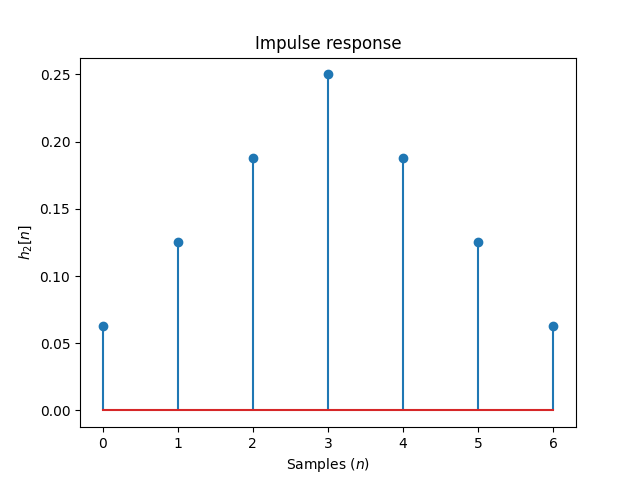
\includegraphics[width=7.5cm, height=6.5cm]{ch10/figures/h2.png}
                  \caption{Impulse response for $y_{2}[n]$}
                  \label{h2}
                \end{marginfigure}
        \end{enumerate}

  % Exercise 3
  \item

        \begin{enumerate}[a)]
          % Exercise 3a)
          \item The output signal $y[n]$ will have the same length as $x[n]$, thus, computing each value
                is done as follows:
                \begin{align*}
                  y[0] & = \frac{1}{1}(x[0 - 0] + x[0 - 1] + x[0 - 2]), \\
                  y[1] & = \frac{1}{2}(x[1 - 0] + x[1 - 1] + x[1 - 2]), \\
                  y[2] & = \frac{1}{3}(x[2 - 0] + x[2 - 1] + x[2 - 2]), \\
                  y[3] & = \frac{1}{3}(x[3 - 0] + x[3 - 1] + x[3 - 2]), \\
                  y[4] & = \frac{1}{3}(x[4 - 0] + x[4 - 1] + x[4 - 2]),
                \end{align*}
                Note that the values of factor in front varies. The reason is that the operation is to average,
                so we must divide by the total number of terms that are counted. Remove all the negative index
                terms (which are treated as 0), we get:
                \begin{align*}
                  y[0] & = \frac{1}{1}(x[0 - 0]) = x[0] = 1.2,                                                   \\
                  y[1] & = \frac{1}{2}(x[1 - 0] + x[1 - 1]) = \frac{1}{2}(x[1] + x[0]) = 2.75,                   \\
                  y[2] & = \frac{1}{3}(x[2 - 0] + x[2 - 1] + x[2 - 2]) = \frac{1}{3}(x[2] + x[1] + x[0]) = 3.40, \\
                  y[3] & = \frac{1}{3}(x[3 - 0] + x[3 - 1] + x[3 - 2]) = \frac{1}{3}(x[3] + x[2] + x[1]) = 4.10, \\
                  y[4] & = \frac{1}{3}(x[4 - 0] + x[4 - 1] + x[4 - 2]) = \frac{1}{3}(x[4] + x[3] + x[2]) = 3.63,
                \end{align*}
                so the filtered signal $y[n]$ is then:
                \[
                  y[n] = \begin{cases}
                    1.2, \quad n = 0,  \\
                    2.75, \quad n = 1, \\
                    3.40, \quad n = 2, \\
                    4.10, \quad n = 3, \\
                    3.63, \quad n = 4.
                  \end{cases}
                \]

          % Exercise 3b)
          \item Listing \ref{ra:solution_b} shows a Python implementation that implements the
                running average filter from Equation \ref{eq:ex:filter}.
                Running this code on the signal $x[n]$ gives the same result as the
                computation done in the previous exercise.
                \lstinputlisting[language=Python, caption=Solution for exercise 3b, label=ra:solution_b]{ch10/code/ex10_3b.py}

          % Exercise 3c)
          \item Listing \ref{ra:solution_c} shows the previous function added to the code from Listing \ref{ch10:precode1}
                \lstinputlisting[language=Python, caption=Solution for exercise 3c, label=ra:solution_c, linerange={0-50}]{ch10/code/ex10_3c.py}
                The plot generated is shown in Figure \ref{ch10:fig:ex3c}.
                Note that the plot is random, so yours will look different when the code is run.

                \begin{marginfigure}
                  \begin{center}
                    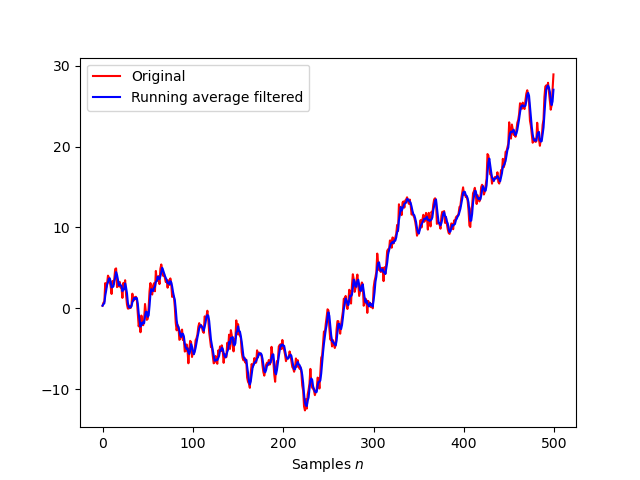
\includegraphics[width=6.9cm, height=7.0cm]{ch10/figures/ex10_3c.png}
                    \caption{Noisy signal that has been smoothened with a running average
                      filter using $L=25$.}
                    \label{ch10:fig:ex3c}
                  \end{center}
                \end{marginfigure}

          % Exercise 3d)
          \item The code in Listing \ref{ch10:code:ex10_3d} implements the running average filter
                and applies the running average filter to the input file. The code is written
                so that the user can run the code by providing the filename and $L$ on the command line.
                \lstinputlisting[language=Python, caption=Suggested solution for exercise 3d, label=ch10:code:ex10_3d]{ch10/code/ex10_3d.py}

                The effect on the audio can be heard between the original and for large $L$. 
                The higher frequencies have been reduced, so they are less prevalent. 
                This is not surprising, as the filter we are using is a low-pass filter. 

        \end{enumerate}

  % Exercise 4
  \item The code for this exercise is based on the reverb demonstration code. 
        \begin{enumerate}[a)]
          % Exercise 4a)
          \item By running \verb|reverb.py| and listening to \verb|reverb.wav|, one can
                hear the reverb effect having been applied to the audio-signal.

          % Exercise 4b)
          \item Running the code in Listing \ref{ex10_4b:code} yields the figure shown in Figure \ref{fig:ex_4b}.
                Each peak shown represents an impulse that has been reflected by some wall, except the first
                peak, which represents the original signal.
                \begin{marginfigure}
                  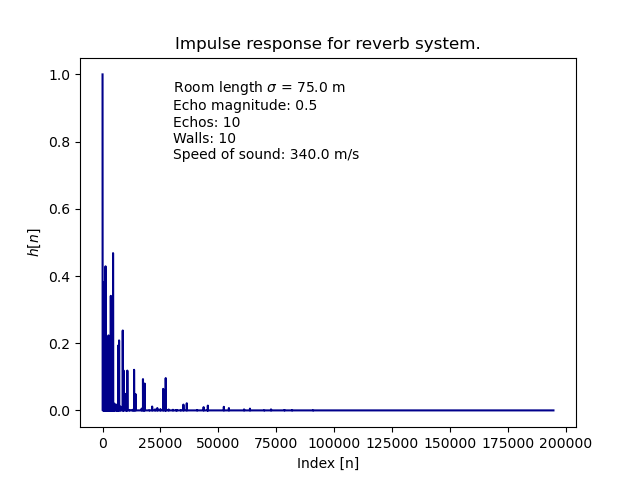
\includegraphics[width=6.9cm, height=7.0cm]{ch10/figures/ex10_4b.png}
                  \caption{Impulse response for the reverb LTI system.}
                  \label{fig:ex_4b}
                \end{marginfigure}

                \lstinputlisting[language=Python, caption=Suggested solution for exercise 4b, label=ex10_4b:code, linerange={0-111}]{ch10/code/ex10_4b.py}

          % Exercise 4c)
          \item By changing \verb|room_length_std| one can increase the reverb effect.
                Making this parameter larger means the sound will travel further and reflect at a later time.
                This gives the effect of a larger room. The impulse responses are similar,
                but the impulse response for a larger room has more peaks at higher indices. This makes
                sense, as the smaller room will not have any reflections on these indices as they do not exist
                for the small room. That is, there are no walls to reflect off of at such distances.
                Running Listing \ref{ex10_4c:code} gives Figure \ref{fig:ex10_4c}, where we can see that
                the larger room has more peaks at higher indices than the smaller room. You can also
                see that the smaller room has more peaks at lower indices, which is as expected as these
                reflections come earlier, due to the signal having less travel distance, than in the large room.

                \begin{marginfigure}
                  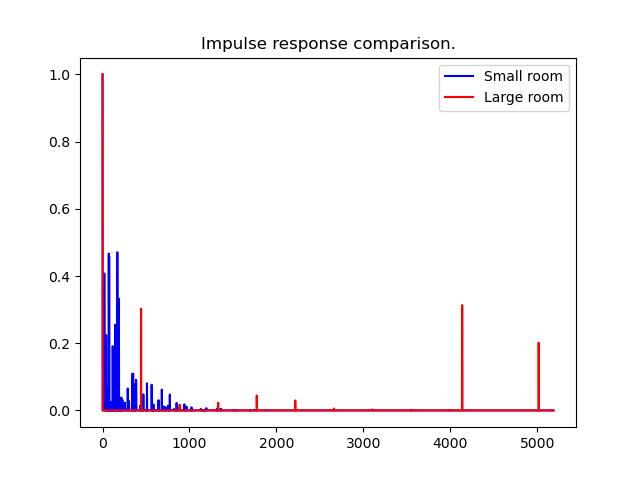
\includegraphics[width=6.9cm, height=7.0cm]{ch10/figures/ex10_4c.png}
                  \caption{Impulse response for the reverb LTI system.}
                  \label{fig:ex10_4c}
                \end{marginfigure}

                \lstinputlisting[language=Python, caption=Suggested solution for exercise 4b, label=ex10_4c:code, linerange={0-49}]{ch10/code/ex10_4c.py}

          % Exercise 4d)
          \item The impulse response $h[n] = \delta[n] + 0.5\delta[n - n_0]$ represents a system
                where the original signal is unchanged, this can be seen from the $\delta[n]$ term. In addition,
                there is the $0.5\delta[n - n_0]$ term, which represents the original signal being delayed
                and reduced by a factor of 0.5 in amplitude. We want this to represent a delay of an echo
                from a 1000 meters distance. To do this, we must find $n_0$ so that the distance traveled by
                the echo is 1000 meters. Assuming a constant velocity for the audio signal, the total time it takes
                for the signal to travel, bounce off a wall and come back is then:
                \[ t = \frac{2s}{v} \]
                where $s = 1000\ \text{m}$ and $v = 343\ \text{m/s}$ (the assumed speed of sound).
                The relation between time in seconds and samples for a discretized signal is then:
                \[ t = T_{s}n. \]
                Solving for $n_{0}$, we obtain:
                \[ n_{0} = \frac{2s}{T_{s}v} = \frac{2sf_{s}}{v}, \]
                where $f_{s}$ is the sample rate. Plugging in the numbers yields:
                \[ n_{0} = \frac{2sf_s}{v}=\frac{(2)(1000\ \text{m})(44100)\ \text{Hz}}{343\ \text{m/s}}\approx257142.85, \]
                or $n_{0} = 257143$ to round to the nearest integer. 
                The implementation of this reverb effect is shown in Listing \ref*{ex10_4d:code}. 
                The delay should occur at 
                \[ t = T_{s}n = n/f_{s} = 257143/44100\ \text{Hz} = 5.83\ \text{seconds}.\]
                If you listen to the audio produced by the code, you should be able to hear the delay coming in at
                around 5.83 seconds, as hoped.
                
                \lstinputlisting[language=Python, caption=Solution for exercise 4, label=ex10_4d:code, linerange={0-83}]{ch10/code/ex10_4d.py}

        \end{enumerate}

\end{enumerate}